%%%%%%%%%%%%%%%%%%%% Revised version -- MCCSAI 2026 (svproc) %%%%%%%%%%%%%%%%%%%%
\documentclass{svproc}

\usepackage{url}
\usepackage{amsmath,amssymb,amsfonts}
\usepackage{graphicx}
\usepackage{booktabs}
\usepackage{multirow}
\usepackage{xcolor}
\def\UrlFont{\rmfamily}

\begin{document}
\mainmatter

\title{Evaluating Time Series Foundation Models for Remaining Useful Life
Prediction: A Comparative Study of Chronos-1 and Chronos-2}
\titlerunning{Chronos-1 vs Chronos-2 for RUL Prediction (extended)}
\author{}
\institute{}
\maketitle

\begin{center}\fbox{\parbox{0.92\textwidth}{\small\textit{Extended version kept as a
research record. It complements the 8-page conference version with the full
multi-seed grid (including the XGBoost head), re-run baselines, the statistical
analysis and reproducibility notes (Sect.~4.5 and~6). Results: run of
2 November 2026, notebook \texttt{W09\_FD001\_MultiSeed\_Stats.ipynb}.}}}\end{center}

\begin{abstract}
Knowing how long an industrial asset can keep operating before it fails,
its Remaining Useful Life, is central to predictive maintenance. Deep
models trained for this task, however, need large amounts of rare
run-to-failure data and must be retrained whenever the monitored system
changes. Foundation models pretrained on generic time series offer an
alternative, since their representations can be reused as they are. This
paper studies when such representations are useful for life prediction,
by comparing the univariate Chronos-1 and the multivariate Chronos-2 on
the NASA turbofan engine benchmark. Both models are kept frozen, and
their outputs are passed to lightweight regressors under several pooling
and sensor selection strategies. Over five random seeds, the best Chronos-2 configuration reaches an RMSE
of 14.61 $\pm$ 0.17 cycles, improving on Chronos-1 (14.92) and coming close
to a task-specific recurrent network trained under the same protocol
(13.93 $\pm$ 0.90), without statistically significant difference. Keeping a diverse set of sensors also matters more than keeping
only the most predictive ones (14.61 vs.\ 19.16).
\keywords{Time series foundation models, Predictive maintenance,
Remaining useful life, Transfer learning, Chronos}
\end{abstract}

\section{Introduction}

Predictive maintenance (PdM) aims to minimise unplanned downtime and
maintenance costs~\cite{khan2018}. At its core lies the estimation of the
Remaining Useful Life (RUL), which allows engineers to move from reactive
interventions to condition-driven strategies. Its impact extends
beyond maintenance, since an unexpected failure quickly turns into
production losses and contractual penalties.

Today, the most accurate RUL predictors are deep networks trained for one
specific asset. Their strength is also their weakness: they require
labelled run-to-failure trajectories, which are rare and costly to
collect, and they must be retrained when the target system changes. Time
Series Foundation Models (TSFMs) approach the problem from the opposite
direction. Pretrained once on large and diverse corpora, they provide
generic temporal representations that can be reused without retraining
the backbone~\cite{chronos2024}. Within Amazon's Chronos family, Chronos-1 is univariate and therefore ignores the
dependencies between sensors, whereas Chronos-2~\cite{chronos2_2025}
processes several variables jointly through group attention. Whether, and
under which design choices, these frozen representations are useful for
RUL regression is still poorly understood.

This paper addresses this question through a controlled evaluation of
frozen Chronos-1 and Chronos-2 representations on C-MAPSS FD001. Our
contributions are:
\begin{enumerate}
\item a comparison of Chronos-1 and Chronos-2 under a protocol identical
  to a published Chronos-1 study~\cite{imsa2025}, so that differences can
  be attributed to the backbone;
\item a systematic exploration of the design space of frozen embeddings
  (pooling strategy, regression head and feature selection);
\item evidence that feature diversity, rather than individual feature
  relevance, drives Chronos-2 performance.
\end{enumerate}

The remainder of this paper is organized as follows. Section~2 reviews
related work. Section~3 describes the methodology. Section~4 presents
experimental results. Section~5 discusses key findings, Section~6 gathers
reproducibility notes, and Section~7 concludes the paper.

\section{Related Work}

This section reviews task-specific deep learning for RUL prediction, then
introduces time series foundation models, and finally discusses how
these models have been applied to RUL prediction.

\textit{Task-specific deep learning for RUL.} Model-based approaches rely
on physical degradation models, which are difficult to build for complex
systems~\cite{khan2018}; this difficulty has motivated data-driven
alternatives, starting with recurrent networks~\cite{heimes_recurrent_2008}.
Convolutional networks (CNNs) were then applied to sensor
windows~\cite{babu2016}, and deeper 1-D CNNs reached an RMSE of 12.61 on
FD001~\cite{li2018}, although convolutions only capture local temporal
context. Long short-term memory networks (LSTMs)~\cite{hochreiter1997}
overcome this limitation by modelling long-range dependencies and have
become a standard for RUL prediction~\cite{zheng2017}, sometimes combined
with CNNs in hybrid architectures~\cite{zhao2020}. Whatever their
architecture, however, these models are trained from scratch for one
dataset and must be retrained when the system changes.

\textit{Time series foundation models.} TSFMs were introduced precisely
to avoid this repeated training. Pretrained on heterogeneous time series,
they differ mainly in how they represent the input. Chronos~\cite{chronos2024} scales and quantises values into tokens
and trains T5 language models with a cross-entropy loss, while
TimesFM~\cite{das2024timesfm} is a decoder-only transformer operating on
patches. MOIRAI~\cite{woo2024moirai} relies on any-variate attention to
handle a variable number of channels. MOMENT~\cite{goswami2024moment}, pretrained by masked
reconstruction, explicitly targets representation learning. Finally,
Chronos-2~\cite{chronos2_2025} is an encoder that processes groups of
related series jointly through group attention. Being pretrained for forecasting or reconstruction, all of them require
a transfer step to be applied to RUL.

\textit{TSFMs for RUL prediction.} Several recent works have explored
such transfer. A first study~\cite{imsa2025} used frozen Chronos-1
embeddings, extracted sensor by sensor, with XGBoost and MLP heads on
FD001; a task-specific LSTM nevertheless remained better (RMSE 14.32 vs.\
14.92). Dint\'en and Zorrilla~\cite{dinten2025} followed a similar idea
with MOMENT embeddings and classical regressors, showing benefits in
few-shot settings. Concurrently with the present work, Abdouni et
al.~\cite{abdouni2026} went further by adding a trainable
compress-and-flatten adapter on top of Chronos-2 and a Wide~\&~Deep head
fed with handcrafted features, reaching 9.97 on FD001 (10.68 without the
handcrafted branch). To our knowledge, TimesFM and MOIRAI
have not yet been evaluated for RUL on C-MAPSS. None of these studies examines how pooling, regression
head and feature selection interact with a frozen multivariate backbone;
this is the gap addressed here. For this reason, \cite{imsa2025} serves
as the primary baseline: it shares our preprocessing, window, RUL cap,
heads and evaluation protocol, and is therefore the only reference for
which the Chronos-1/Chronos-2 difference is not confounded by protocol
differences.

\section{Methodology}

Building on this positioning, the evaluated pipeline comprises four steps
(Fig.~\ref{fig:methodology}): problem formulation, feature selection,
frozen embedding extraction and regression.

\begin{figure}[t]
\centering
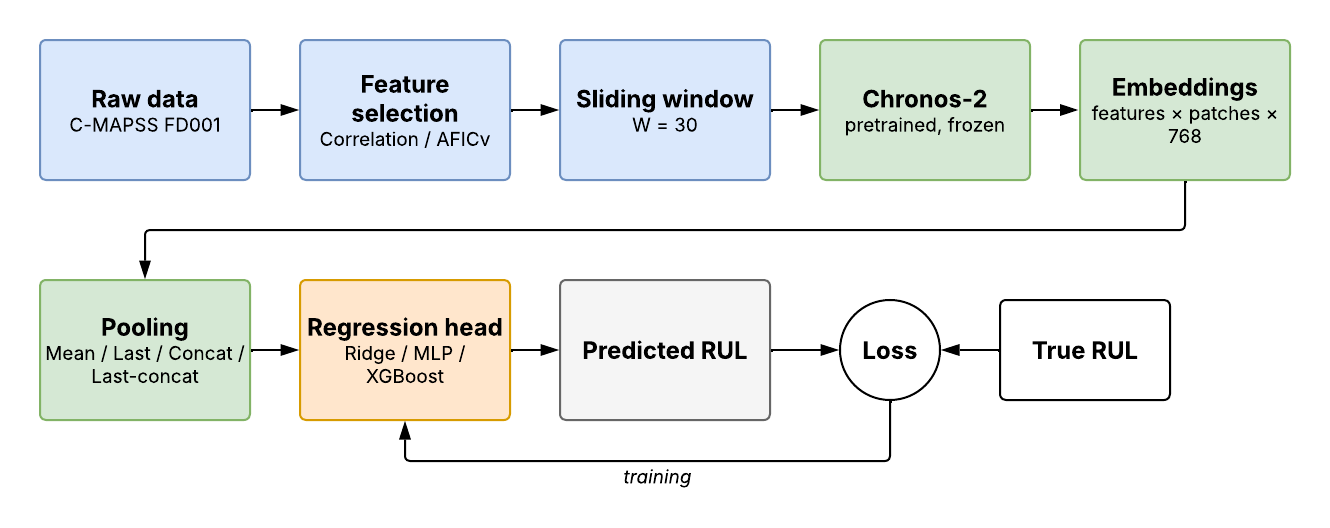
\includegraphics[width=0.9\textwidth]{methodology_diagram.png}
\caption{Overview of the evaluated pipeline.}
\label{fig:methodology}
\end{figure}

\subsection{Problem Formulation}

Given multivariate readings $\mathbf{X} = \{x_1, \ldots, x_T\}$,
$x_t \in \mathbb{R}^d$, of an engine failing at cycle $T$, the target is
the piecewise-linear RUL $y_t = \min(T - t,\; R_\text{max})$ with
$R_\text{max} = 125$~\cite{cmapss}. A sliding window of $W = 30$ cycles
is used to predict the RUL at its last cycle. This value is the standard
choice for FD001~\cite{li2018}; it is also the largest window compatible
with the shortest test trajectory (31 cycles), so every test engine can
be evaluated without padding.

\subsection{Feature Selection}

FD001 provides 24 raw variables (21 sensors and 3 operating settings),
min-max normalised with statistics fitted on the training set. Two
strategies are compared to select the model inputs
(Table~\ref{tab:features}). The \textit{correlation-based} strategy aims
at a diverse, non-redundant set: it removes near-constant variables, then
one variable of each highly correlated pair. In contrast,
\textit{AFICv}~\cite{Alomari2023Advancing} focuses on individual
relevance, keeping the smallest subset of variables that covers 90\% of
the cumulative gain importance of an XGBoost regressor fitted on the
training set.

\begin{table}[t]
\caption{Effect of the two feature selection strategies on the number
of input variables (FD001).}
\label{tab:features}
\centering\small
\begin{tabular}{@{}llccc@{}}
\toprule
\textbf{Step} & \textbf{Criterion} & \textbf{Input} & \textbf{Removed} & \textbf{Output} \\
\midrule
\multicolumn{5}{@{}l}{\textit{Correlation-based strategy}} \\
\quad Variance filter & variance $< 0.001$ & 24 & 7 & 17 \\
\quad Correlation filter & $|\rho| > 0.95$ & 17 & 1 & \textbf{16} \\
\midrule
\multicolumn{5}{@{}l}{\textit{AFICv strategy}} \\
\quad Importance ranking & 90\% cum.\ importance & 24 & 16 & \textbf{8} \\
\bottomrule
\end{tabular}
\end{table}

\subsection{Embedding Extraction}

The selected variables are then encoded by one of the two frozen
backbones. \textit{Chronos-1} (\texttt{chronos-t5-small}, 46M parameters)
is univariate, so each sensor window $\mathbf{W}_{:,i} \in \mathbb{R}^{W}$
is encoded separately and averaged over time, and the $d$ sensor
embeddings are concatenated:
\begin{equation}
\mathbf{e} = \big[\,\text{MeanPool}(\text{Chronos-1}(\mathbf{W}_{:,i}))\,\big]_{i=1}^{d}.
\end{equation}
By construction, this representation cannot capture cross-sensor
dependencies. \textit{Chronos-2} (\texttt{amazon/chronos-2}, 120M
parameters) removes this limitation by encoding all $d$ variables jointly
through group attention. Its output is a tensor of shape
$(d,\, n_\text{patches},\, d_\text{model}{=}768)$, which must be reduced
to a vector $\mathbf{e} = \text{Pool}(\text{Chronos-2}(\mathbf{W}))$. Four
pooling strategies are compared for this purpose: \textit{mean} (average
over variables and patches, 768 dimensions), \textit{last} (last patch,
averaged over variables, 768), \textit{concat} (average over variables,
patches concatenated, 3,072) and \textit{last-concat} (last patch of each
variable concatenated, 12,288).

\subsection{Regression Heads and Evaluation}

Finally, three heads map $\mathbf{e}$ to the estimate $\hat{y}_t$, as
in~\cite{imsa2025}: a linear \textit{Ridge} regression ($\alpha = 1$), a
non-linear \textit{MLP} (256 and 128 ReLU units, Adam, early stopping on
10\% of the training windows) and \textit{XGBoost} (100 trees, depth 5).
The main text focuses on Ridge and MLP; XGBoost results, which proved
sensitive to the library version (Sect.~6), are reported in Sect.~4.5. Only the head is trained. Performance is measured on the last window of each test
engine by $\text{RMSE} = \sqrt{\tfrac{1}{N}\sum_{i}(y_i - \hat{y}_i)^2}$
and by the NASA score $S = \sum_i s_i$, with $s_i = e^{-d_i/13} - 1$ if
$d_i < 0$ and $e^{d_i/10} - 1$ otherwise, where
$d_i = \hat{y}_i - y_i$~\cite{saxena2008}; the score penalises late
predictions more heavily, as they are the most dangerous in practice.

\section{Experiments and Results}

This section first describes the dataset and experimental setup, then
analyses the impact of the pooling strategy, the regression head and the
feature selection, and finally compares the best configuration with LSTM
baselines and other Chronos-based models.

\subsection{Experimental Setup}

The experiments use C-MAPSS FD001~\cite{cmapss}, which contains 100
training engines run to failure (20,631 cycles) and 100 test engines
truncated before failure (13,096 cycles), with the true RUL provided for
the latter, under one operating condition and one fault mode. Windowing
yields 17,731 training and 10,196 test windows, and the last window of
each of the 100 test engines is scored. FD001 is the smallest C-MAPSS
subset (FD002 and FD004 contain 260 and 249 training engines), a
small-data regime where transferable representations should help. Chronos embeddings are
deterministic, as is the Ridge head. The MLP head and a task-specific
baseline (two-layer LSTM with 64 units, trained end to end on the same
windows with early stopping) are trained with five random seeds (42, 123,
456, 789, 1000), and results are reported as mean $\pm$ standard
deviation. Embeddings are extracted on a T4 GPU.

\subsection{Pooling Strategy and Regression Head}

The first experiment identifies how the Chronos-2 output should be
summarised (Table~\ref{tab:pooling}, correlation-based features).

\begin{table}[t]
\centering\small
\begin{minipage}[t]{0.48\textwidth}\centering
\caption{Chronos-2 RMSE by pooling and head (correlation features).
$^\dagger$Single run.}
\label{tab:pooling}
\begin{tabular}{@{}lccc@{}}
\toprule
\textbf{Pooling} & \textbf{Dim} & \textbf{Ridge} & \textbf{MLP} \\
\midrule
Mean        & 768    & 15.68 & \textbf{14.61}\,$\pm$\,0.17 \\
Last        & 768    & \textbf{15.20} & 15.21\,$\pm$\,0.23 \\
Concat      & 3,072  & 15.49 & 15.07\,$\pm$\,0.23 \\
Last-concat$^\dagger$ & 12,288 & -- & 18.03 \\
\bottomrule
\end{tabular}
\end{minipage}\hfill
\begin{minipage}[t]{0.48\textwidth}\centering
\caption{Chronos-2 (mean pooling) by feature set and head.}
\label{tab:results}
\begin{tabular}{@{}llcc@{}}
\toprule
\textbf{Feat.} & \textbf{Head} & \textbf{RMSE} & \textbf{Score} \\
\midrule
Corr. & MLP   & \textbf{14.61}\,$\pm$\,0.17 & \textbf{358}\,$\pm$\,30 \\
Corr. & Ridge & 15.68 & 388 \\
\midrule
AFICv & MLP   & 19.16\,$\pm$\,0.48 & 939\,$\pm$\,129 \\
AFICv & Ridge & 19.03 & 772 \\
\bottomrule
\end{tabular}
\end{minipage}
\end{table}

Mean pooling with the MLP gives the lowest RMSE and is retained for the
next experiments. Interestingly, the linear Ridge head prefers the
last patch (15.20) to the mean (15.68), the opposite of the MLP.

\subsection{Feature Selection}

With the pooling fixed, the second experiment compares the two feature
sets across both heads (Table~\ref{tab:results}). The gap is large and
consistent: whatever the head, correlation-based selection outperforms
AFICv by at least 3.3 cycles, far beyond the seed-to-seed variability.

\subsection{Comparison with LSTM and Chronos-Based Models}

The best configuration can now be positioned against the LSTM baselines
and the other Chronos-based models (Table~\ref{tab:baselines}). The upper
block gathers models evaluated under the identical protocol, so that
differences reflect the models themselves. The lower block reports the
concurrent Chronos-2 models of~\cite{abdouni2026}, which use a different
training pipeline and are given for reference.

\begin{table}[t]
\caption{Comparison of LSTM baselines and Chronos-based models on FD001.
Upper block: identical protocol (mean $\pm$ std over five seeds for
re-trained models; $^\ast$values reported in~\cite{imsa2025}). Lower block: trained adapter on Chronos-2,
different protocol (values as reported).}
\label{tab:baselines}
\centering
\begin{tabular}{lcc}
\toprule
\textbf{Method} & \textbf{RMSE} & \textbf{Score} \\
\midrule
Task-specific LSTM (re-trained)         & \textbf{13.93~$\pm$~0.90} & 378.6~$\pm$~100.0 \\
Task-specific LSTM$^\ast$               & 14.32 & \textbf{325.1} \\
Chronos-2 + MLP, mean (ours)            & 14.61~$\pm$~0.17 & 357.9~$\pm$~30.4 \\
Chronos-1 + MLP$^\ast$                  & 14.92 & 641.6 \\
Chronos-2 + Ridge, last (ours)          & 15.20 & 349.8 \\
Chronos-1 + XGBoost$^\ast$              & 15.93 & 379.0 \\
Classical LSTM$^\ast$                   & 16.14 & 397.8 \\
\midrule
Chronos-2 + adapter, deep only~\cite{abdouni2026}  & 10.68~$\pm$~0.34 & -- \\
Chronos-2 + adapter, Wide\&Deep~\cite{abdouni2026} & 9.97~$\pm$~0.34 & 187.4 \\
\bottomrule
\end{tabular}
\end{table}


\subsection{Extended Results and Statistical Analysis}

This subsection gathers all results of the multi-seed run, including the
XGBoost head and baselines re-trained under the identical protocol, as a
reference for future work.

\begin{table}[h]
\caption{Full Chronos-2 grid on FD001 (RMSE, mean $\pm$ std over five seeds;
Ridge and XGBoost are deterministic). Corr.: correlation-based features (16);
AFICv: 8 features.}
\label{tab:fullgrid}
\centering\small
\begin{tabular}{@{}llcccc@{}}
\toprule
\textbf{Feat.} & \textbf{Pooling} & \textbf{Dim} & \textbf{Ridge} & \textbf{MLP} & \textbf{XGBoost} \\
\midrule
Corr.  & Mean   & 768   & 15.68 & \textbf{14.61}\,$\pm$\,0.17 & 16.97 \\
Corr.  & Last   & 768   & 15.20 & 15.21\,$\pm$\,0.23 & 17.11 \\
Corr.  & Concat & 3,072 & 15.49 & 15.07\,$\pm$\,0.23 & 15.87 \\
\midrule
AFICv  & Mean   & 768   & 19.03 & 19.16\,$\pm$\,0.48 & 20.36 \\
AFICv  & Last   & 768   & 18.49 & 19.40\,$\pm$\,0.26 & 21.19 \\
AFICv  & Concat & 3,072 & 19.39 & 18.59\,$\pm$\,0.36 & 20.33 \\
\bottomrule
\end{tabular}
\end{table}

\begin{table}[h]
\caption{Baselines re-trained under the identical protocol (five seeds).
Chronos-1 uses mean pooling over time and correlation-based features.}
\label{tab:rerun}
\centering\small
\begin{tabular}{@{}lccc@{}}
\toprule
\textbf{Model} & \textbf{RMSE} & \textbf{Range} & \textbf{Score} \\
\midrule
XGBoost on raw windows (480 inputs) & \textbf{13.63} & -- & 339.3 \\
Task-specific LSTM (2$\times$64)    & 13.93\,$\pm$\,0.90 & 13.10--15.37 & 378.6\,$\pm$\,100.0 \\
Chronos-2 + MLP, mean               & 14.61\,$\pm$\,0.17 & 14.39--14.84 & 357.9\,$\pm$\,30.4 \\
Chronos-1 + Ridge                   & 15.68 & -- & 361.0 \\
Chronos-1 + XGBoost                 & 17.52 & -- & 563.9 \\
Chronos-1 + MLP                     & 18.19\,$\pm$\,0.32 & 17.93--18.75 & 685.5\,$\pm$\,12.1 \\
\bottomrule
\end{tabular}
\end{table}

To assess the significance of the differences, predictions were averaged
over seeds and compared with the reference configuration (Chronos-2 + MLP,
mean pooling, correlation features) on the 100 test engines, using 95\%
bootstrap confidence intervals (5,000 resamples) and paired Wilcoxon
signed-rank tests on per-engine absolute errors (Table~\ref{tab:stats}).

\begin{table}[h]
\caption{Statistical comparison with Chronos-2 + MLP (mean, correlation).
RMSE of seed-averaged predictions, 95\% bootstrap CI, difference in RMSE
with its 95\% CI, and paired Wilcoxon $p$-value.}
\label{tab:stats}
\centering\small
\begin{tabular}{@{}lcccc@{}}
\toprule
\textbf{Configuration} & \textbf{RMSE} & \textbf{95\% CI} & \textbf{$\Delta$RMSE [95\% CI]} & \textbf{$p$} \\
\midrule
Chronos-2 + MLP, mean (ref.)   & 14.49 & [12.47, 16.47] & -- & -- \\
XGBoost on raw windows         & 13.63 & [11.37, 15.88] & $-$0.86 [$-$3.90, 2.27] & 0.264 \\
Task-specific LSTM             & 13.53 & [11.21, 15.77] & $-$0.97 [$-$3.63, 1.63] & 0.115 \\
Chronos-2 + MLP, concat        & 14.80 & [12.77, 16.70] & 0.31 [$-$0.85, 1.45] & 0.195 \\
Chronos-2 + Ridge, last        & 15.21 & [13.38, 17.00] & 0.71 [$-$0.57, 2.03] & 0.156 \\
Chronos-2 + Ridge, mean        & 15.68 & [13.74, 17.53] & 1.19 [0.19, 2.23] & 0.040 \\
Chronos-1 + Ridge              & 15.68 & [13.82, 17.44] & 1.19 [$-$1.54, 3.86] & 0.128 \\
Chronos-1 + MLP                & 17.94 & [14.98, 20.65] & 3.45 [0.10, 6.91] & 0.552 \\
Chronos-2 + MLP, mean, AFICv   & 19.01 & [15.98, 21.75] & 4.52 [2.44, 6.42] & 0.007 \\
Chronos-2 + Ridge, mean, AFICv & 19.03 & [16.37, 21.61] & 4.54 [2.59, 6.41] & $<$0.001 \\
\bottomrule
\end{tabular}
\end{table}

Three observations complement the main results. First, none of the
task-specific baselines is significantly better than Chronos-2 + MLP: the
confidence intervals of the differences all contain zero, which reflects
the limited size of the FD001 test set (100 engines). Second, every AFICv
configuration is significantly worse than the reference ($p \le 0.033$ for
all heads and poolings), which makes the feature diversity effect the most
robust finding of the study. Third, the XGBoost head is consistently the
weakest head on Chronos-2 embeddings, and Chronos-1 + MLP is clearly worse
than Chronos-2 + MLP, although the difference only borders on
significance (CI lower bound 0.10).

\section{Discussion}

This section interprets the results and their practical implications.

\textit{Pooling strategy.} As seen in Table~\ref{tab:pooling}, compact
mean pooling suits the MLP best, whereas the Ridge head performs best with
the last patch, which reflects the most recent degradation state and is
easier to exploit linearly. The MLP, in contrast, benefits from a summary
of the whole window, and the very high-dimensional last-concat
representation degrades it markedly. Pooling and head should therefore be
chosen jointly.

\textit{Feature selection.} The feature selection results point in the
same direction. As Table~\ref{tab:features} shows, AFICv keeps only
half as many variables (8 vs.\ 16), retaining the individually most
predictive ones, some of which are strongly correlated with each other,
while discarding sensors that are weak in isolation yet provide context
to Chronos-2's group attention. For a multivariate foundation model,
diversity of the input group thus matters more than individual relevance.

\textit{Chronos-2 vs.\ Chronos-1.} Under the same protocol, Chronos-2 +
MLP improves on both Chronos-1 + MLP (14.61 vs.\ 14.92) and Chronos-1 +
XGBoost (15.93), with a markedly better NASA score (357.9 vs.\ 641.6).
This consistent trend supports joint multivariate encoding over
per-sensor concatenation.

\textit{Why use a frozen foundation model?} Compared with the
task-specific LSTM, the remaining gap is small (14.61 vs.\ 13.93) and
not statistically significant (paired Wilcoxon test on the 100 test
engines, $p = 0.12$); the frozen approach is also much more
stable across seeds ($\pm$\,0.17 vs.\ $\pm$\,0.90). The
frozen approach, however, only trains a lightweight head on embeddings
that are computed once, instead of designing and training a recurrent
architecture end to end, and the same backbone and embeddings can be
reused across assets.

The adapter-based Chronos-2 models of~\cite{abdouni2026} clearly
outperform ours (9.97 vs.\ 14.61), but the two studies answer different
questions, and our results remain informative for three reasons. First,
their gain comes from components trained specifically for RUL: a learned
adapter, a Wide~\&~Deep head and handcrafted features. Ours involves none of
these and measures what the frozen representation alone provides, so the
gap between the two (14.61 vs.\ 10.68 without handcrafted features)
quantifies the value of task-specific adaptation. Second, our findings concern choices made
upstream of any head and thus transfer to such pipelines: the
compress-and-flatten adapter is itself a learned pooling, consistent with our
finding that pooling, like sensor diversity, strongly affects
performance. Third, the frozen approach is the cheapest to deploy across many
asset types with little labelled data. The two are thus complementary.

\textit{Limitations.} These conclusions are limited to FD001, which
involves a single operating condition.

\section{Reproducibility Notes}

The following points are recorded to ease the reproduction and extension of
this study.

\textit{Software versions.} The multi-seed run used xgboost 3.4.1,
scikit-learn 1.6.1, PyTorch 2.11.0 and chronos-forecasting 2.3.2
(\texttt{amazon/chronos-2}, 119.5M parameters).

\textit{Sensitivity of XGBoost to the library version.} With identical
embeddings (the Ridge head gives exactly the same RMSE, 15.68), XGBoost on
mean-pooled embeddings reached 15.62 in an earlier run (March 2026) and
16.97 in this run. The difference is attributed to changes in the default
behaviour of newer xgboost releases. For the same reason, the AFICv subset
changed slightly (sensor~7 replaces sensor~20), while its size (8
variables) is unchanged. XGBoost results should therefore always be
reported together with the library version.

\textit{Chronos-1 discrepancy.} The re-run Chronos-1 + MLP (18.19) is much
worse than the value reported in~\cite{imsa2025} (14.92), whereas
Chronos-1 + Ridge (15.68) is in line with the other configurations.
Differences in the MLP training (early stopping) and in the embedding
aggregation are the most likely causes; this point should be clarified
before reusing the re-run Chronos-1 values.

\textit{LSTM training.} A first LSTM implementation trained on unscaled
targets diverged for one seed (RMSE 40.4). Scaling the targets to $[0,1]$
by $R_\text{max}$, clipping gradients (norm 1.0) and halving the learning
rate on validation plateaus solved the problem (13.93 $\pm$ 0.90).

\textit{Pooling memory.} The last-concat embeddings (12,288 dimensions)
exceeded the 12.7\,GB RAM of a standard Colab session when cached for the
training windows, which is why this pooling was only evaluated once.

\section{Conclusion}

This paper evaluated frozen Chronos-1 and Chronos-2 representations for
RUL prediction on C-MAPSS FD001 under a controlled protocol. The best
Chronos-2 configuration (mean pooling, MLP head, correlation-based
features) reaches an RMSE of 14.61 $\pm$ 0.17 over five seeds, improves
on Chronos-1 and comes close to a task-specific LSTM trained under the
same protocol (13.93 $\pm$ 0.90), while training only a lightweight head. Beyond
these figures, two lessons emerge: feature diversity is essential for
Chronos-2's group attention, and pooling and head interact strongly
enough to be selected jointly. Building on these results, future work
will address lightweight adaptation and fine-tuning with a RUL-specific loss, the multi-condition
subsets FD002--FD004, and a comparison with other TSFMs such as TimesFM,
MOIRAI and MOMENT under the same protocol.

\bibliographystyle{spmpsci}
\bibliography{bibliography}
\end{document}
